\documentclass[11pt]{scrartcl}
\usepackage{dominatrix}

\usepackage{colortbl}
\usepackage{pgfplots}
\newcommand{\jon}{Jón }
\newcommand{\ve}{\varepsilon}
\pgfplotsset{compat=1.9}
\renewcommand\thesubsection{\alph{subsection}}
\definecolor{light-gray}{gray}{0.75}
\title{Market Efficiency}
\subject{ECON W3213 Spring 2014 \jon Steinsson}
\author{Linan Qiu, lq2137}
\begin{document}

\maketitle

\begin{abstract}
This set of recitation notes covers \textbf{Market Efficiency} (along with some discussions of welfare economics). This is in no way a substitute for attending lectures, but just in case you dozed off or checked your boyfriend's Facebook page while \jon was working Calculus magic on the board, this set of notes may save you.

Happy Valentine's Day everyone!
\end{abstract}

\section{Mindblowing Ideas}
This chapter is more intuition driven than anything else. Here are some intuitive ideas that you must appreciate by the time you finish this chapter.

\begin{itemize}
\item Having \textbf{well defined property rights and competitive markets} for all goods and services results in \textbf{maximum economic efficiency}
\item An allocation is efficient when \textbf{no one can be made better off without making someone else worse off}. We call this \textbf{Pareto Efficiency}. However, this does not address distributional issues. (like inequity!)
\item The \textbf{price} of a good or service in its market is a \textbf{powerful signal} that tells consumers how much to consume and producers how much to produce. The government can attempt to do the same, but will usually fail due to the sheer complexity and scale of such an endeavor.
\end{itemize}

\section{Pareto Efficiency}

\textbf{An allocation is pareto efficient if no one else can be made better off without making someone else worse off.} 

This is how I think about it. Let's say there's only you and me in the world. We both have our utilities, $U_{\mathrm{Linan}}$ and $U_{\mathrm{You}}$. Let me set your utility at a certain level, say $U_{\mathrm{You}} = 10$ At that given level of utility, I will maximize my utility as much as I can until there are no other possible options for me. Once I reach that point, I know that I can't possibly increase my utility $U_{\mathrm{Linan}}$ anymore without decreasing your utility $U_{\mathrm{You}}$.

If I can still improve $U_{\mathrm{Linan}}$ without decreasing $U_{\mathrm{You}}$, this change is said to be a \textbf{pareto improvement}. Obviously, the earlier point is \textbf{pareto inefficient} since I can increase my utility without making you worse off.

There are 3 conditions we use for defining pareto efficiency:

\begin{enumerate}
\item \textbf{Exchange Efficiency}: No further mutually advantageous trade exists
\item \textbf{Production Efficiency}: No further advantageous changes in labor supply exists
\item \textbf{Land Efficiency}: No further advantageous changes in land use exists
\end{enumerate}

\subsection{Robinson Crusoe Model}

In our model, we assume that

\begin{itemize}
\item 2 Consumers, Robinson $R$ and Friday $F$
\item Two inputs to production, labor $L$ and land $N$
\item Two outputs, coconuts $C$ and shelter $S$
\item Start off with endowments of time $\omega_T$ and land $\omega_N$
\item They both have access to two knowledge/technologies:
	\subitem Production function for coconuts: $Y_C = F_C(L_C, N_C)$
	\subitem Production function for shelter: $Y_S = F_S(L_S, N_S)$
\item They consume $X$ of coconuts $C$, shelter $S$, and leisure $Z$
	\subitem Robinson: $U_R(X_{C,R}, X_{S,R}, X_{Z,R})$
	\subitem Friday: $U_F(X_{C,F}, X_{S,F}, X_{Z,F})$
\end{itemize}

\subsection{Exchange Efficiency}

\subsubsection{Marginal Rate of Substitution}

We have seen indifference curves before in your introductory economics courses.

\begin{figure}[H]
\centering
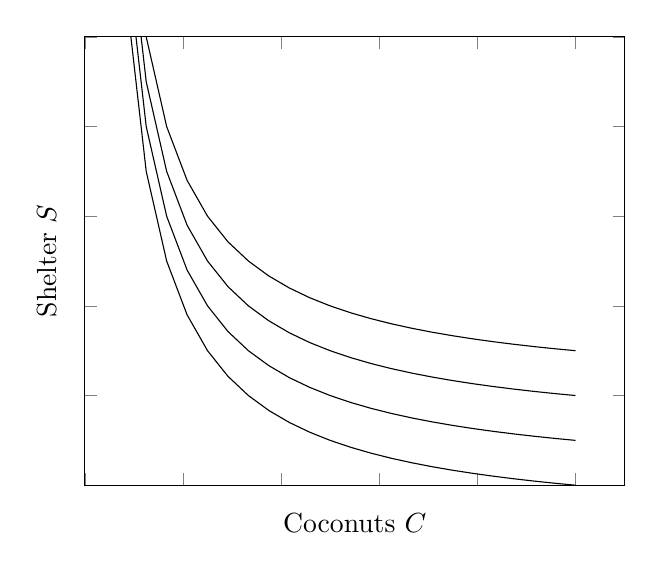
\begin{tikzpicture}
\begin{axis}[yticklabels={,,}, xticklabels={,,},xlabel={Coconuts $C$}, ylabel={Shelter $S$}, ymin=0,ymax=10,xmin=0]

\addplot[black, domain=0:1]
{1/x-1};
\addplot[black, domain=0:1]
{1/x};
\addplot[black, domain=0:1]
{1/x+1};
\addplot[black, domain=0:1]
{1/x+2};

\end{axis}
\end{tikzpicture}
\caption{Indifference Curves of Robinson}
\end{figure}

Due to the lack of proper resources teaching you how to derive the \textbf{Marginal Rate of Substitution}, let's define it proper here.

\[MRS = -\frac{dS}{dC} = \frac{\frac{\partial U}{\partial C}}{\frac{\partial U}{\partial S}}\]

But why? And why the weird flip of $S$ over $C$ to $C$ over $S$? Let's do a little math. Here, we are trying to find the \textbf{total differentiation} of $U_R$. In other words, we're trying to find what happens if we change both $S$ and $C$. You have learnt partial differentiation, where we differentiation $U$ with respect to $S$, holding $C$ constant and vice versa. Now, we are saying, "What if both changes?"

Then we'd need to do something a little different. 

\[dU = \frac{\partial U}{\partial S} dS + \frac{\partial U}{\partial C} dC \]

This says that the change in $U$ should be equal to the change in $U$ contributed from the change in $S$, and the change in $U$ contributed by the change in $C$. I can hear the mathematicians screaming at me, but let's just put them on mute for a while.

Along a single indifference curve, utility doesn't change. So, setting $dU = 0$, 

\begin{align*}
dU &= \frac{\partial U}{\partial S} dS + \frac{\partial U}{\partial C} dC = 0 \\
-\frac{dS}{dC} &= \frac{\frac{\partial U}{\partial C}}{\frac{\partial U}{\partial S}}
\end{align*}

Now what is the MRS? The MRS answers the question, "How many units of shelter can Robinson give up for one additional unit of coconut such that his utility remains the same?"

This is essentially the \textbf{negative} of the slope of the indifference curve (since we are asking for the units of shelter, not negative units of shelter, and the slope is usually negative for indifference curves assuming convex indifference curves)

Hence, 

\[MRS = -\frac{dS}{dC} = \frac{\frac{\partial U}{\partial C}}{\frac{\partial U}{\partial S}}\]

\subsubsection{Defining Exchange Efficiency}

Now let's answer the question, "How will Robinson and Friday distribute coconuts and shelters among themselves?" Another way to phrase this is, "What condition will be true when Robinson and Friday can no longer gain from trading between themselves?"

Let's assume\footnote{We can do the same for coconuts and leisure, shelter and leisure. Basically, this process can apply to all other pairs of goods.}

\begin{itemize}
\item Robinson gives Friday $\epsilon$ coconuts
\item In exchange, Friday gives Robinson $\eta$ shelters
\end{itemize}

Let's begin a distribution that is \textbf{exchange efficient.} In other words, the level that Robinson is consuming right now -- $X^*_{R,C}, X^*_{R,S}, X^*_{R,Z}$ and the level that Friday is consuming -- $X^*_{F,C}, X^*_{F,S}, X^*_{F,Z}$ is pareto optimal. This means that none of them can gain utility from this trade without making the other worse off.

Let $U'_{R,C} = \frac{\partial U_R(X^*_{R,C}, X^*_{R,S}, X^*_{R,Z})}{\partial X_{R,C}}$ In other words, $U'_{R,C}$ is the additional utility gained by Robinson from consuming one more coconut at the consumption level $(X^*_{R,C}, X^*_{R,S}, X^*_{R,Z})$

Let the same apply for Friday.

Then from this transaction,

\begin{table}[ht!]
\begin{longtable}{c|cc}
\hline
 & Robinson & Friday \\
\hline
Marginal Benefit & $U'_{R,C} \epsilon$ & $U'_{F,S} \eta$ \\
Marginal Cost & $U'_{R,S} \eta$ & $U'_{F,C} \epsilon$ \\
\hline
\end{longtable}
\caption{Marginal Costs and Benefits for Robinson and Friday}
\end{table}

Robinson's marginal benefit is the additional utility per coconut (marginal utility of coconut) multiplied by the number of coconuts. However, he's giving friday $\eta$ shelters, hence he loses $-U'_{R,S} \eta$ in utility. A similar argument can be made for Friday.

Now recall the definition of pareto efficiency. If this exchange is not a pareto improvement (ie. the current point $X^*$ is pareto optimal), then neither Robinson's nor Friday's utility should change. That will mean that their marginal benefits and costs are equal.

Hence, using Robinson's marginals,

\begin{align*}
U'_{R,C} \epsilon &= U'_{R,S} \eta \\
\eta &= \frac{U'_{R,C}}{U'_{R,S}} \epsilon
\end{align*}

Substituting $\eta$ into Friday's marginals,

\begin{align*}
U'_{F,S} \eta &= U'_{F,C} \epsilon \\
U'_{F,S} \left( \frac{U'_{R,C}}{U'_{R,S}} \right) \epsilon &= U'_{F,C} \epsilon \\
\frac{U'_{F,S}}{U'_{F,C}} &= \frac{U'_{R,C}}{U'_{R,S}}
\end{align*}

This means that the MRSes of each person should equal each other. This is the condition for exchange efficiency.

Let's see how we can represent this on an \textbf{Edgeworth Box}.

\subsubsection{Edgeworth Box}

An Edgeworth Box represents a certain distribution of two finite goods between two people.



\begin{figure}[H]
\centering
\begin{tikzpicture}
\begin{axis}[yticklabels={,,}, xticklabels={,,},xlabel={Coconuts $C$}, ylabel={Shelter $S$}, ymin=0,ymax=100,xmin=0,xmax=100]

\addplot[mark=*, blue, mark size=3pt, domain=0:100]
coordinates {(50,40)};
\addplot[black,dashed]
coordinates{(0,40) (50,40) (50,0)} node at (axis cs: 10,40) {40} node at (axis cs: 50,10) {50};

% name markings
\addplot[black, domain=0:200]
coordinates {(0,0)} node at (axis cs:20,10) {\color{black} Robinson} node at (axis cs:90,90) {\color{blue} Friday};
\end{axis}
\end{tikzpicture}
\caption{Edgeworth Box of Robinson and \color{blue} Friday}
\end{figure}

For example, this point means that given an initial distribution of 100 shelters and 100 coconuts, Robinson as 40 shelters and 50 coconuts. That leaves Friday with 60 shelters and 50 coconuts. Hence, a single point represents the distribution of two goods between two people. 

You can actually think of this as two of the single person indifference curve diagrams overlaid onto each other. 

\begin{figure}[H]
\centering
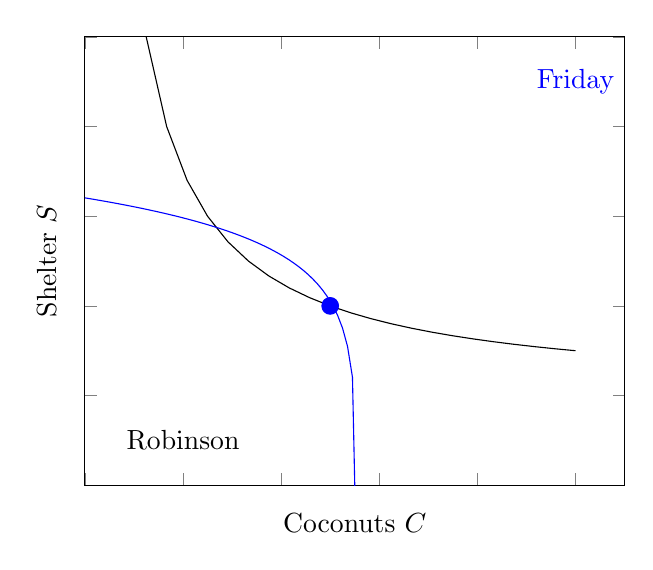
\begin{tikzpicture}
\begin{axis}[yticklabels={,,}, xticklabels={,,},xlabel={Coconuts $C$}, ylabel={Shelter $S$}, ymin=0,ymax=10,xmin=0]

\addplot[mark=*, blue, mark size=3pt, domain=0:100]
coordinates {(0.5,4)};

\addplot[black, domain=0:1]
{1/x+2};

\addplot[blue, domain=0:1,samples=100]
{ln(-9*x+5)+4.8};

% name markings
\addplot[black, domain=0:200]
coordinates {(0,0)} node at (axis cs:0.2,1) {\color{black} Robinson} node at (axis cs:1,9) {\color{blue} Friday};
\end{axis}
\end{tikzpicture}
\caption{Edgeworth Box of Robinson and \color{blue} Friday}
\end{figure}

These are simply their indifference curves. Every point in the diagram corresponds to one of each person's indifference curves. 

Is this distribution exchange efficient? Not really. We can imagine Robinson's indifference curve moving up, and Friday's moving down. This would be preferable to both of them. In other words, any point within this shaded area is preferable to both of them.

\begin{figure}[H]
\centering
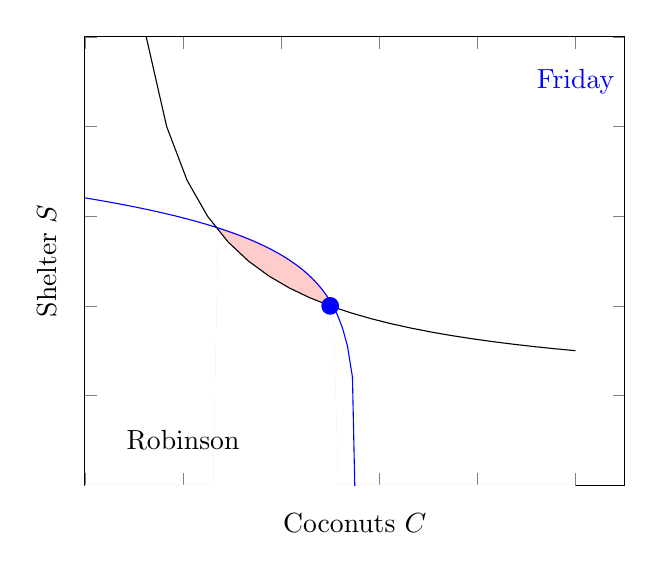
\begin{tikzpicture}
\begin{axis}[yticklabels={,,}, xticklabels={,,},xlabel={Coconuts $C$}, ylabel={Shelter $S$}, ymin=0,ymax=10,xmin=0]

\addplot[fill, red, opacity = 0.2, domain=0:1, samples=100]
{ln(-9*x+5)+4.8 > (1/x+2) ? ln(-9*x+5)+4.8 : 0} \closedcycle;

\addplot[fill, white, domain=0:1, samples=100]
{ln(-9*x+5)+4.8 > (1/x+2) ? (1/x+2) : 0} \closedcycle;

\addplot[mark=*, blue, mark size=3pt, domain=0:100]
coordinates {(0.5,4)};

\addplot[black, domain=0:1]
{1/x+2};

\addplot[blue, domain=0:1,samples=100]
{ln(-9*x+5)+4.8};

% name markings
\addplot[black, domain=0:200]
coordinates {(0,0)} node at (axis cs:0.2,1) {\color{black} Robinson} node at (axis cs:1,9) {\color{blue} Friday};
\end{axis}
\end{tikzpicture}
\caption{Edgeworth Box of Robinson and \color{blue} Friday}
\end{figure}

For example, the point in red could be achieved through mutual exchange, and it will increase both their utility.

\begin{figure}[H]
\centering
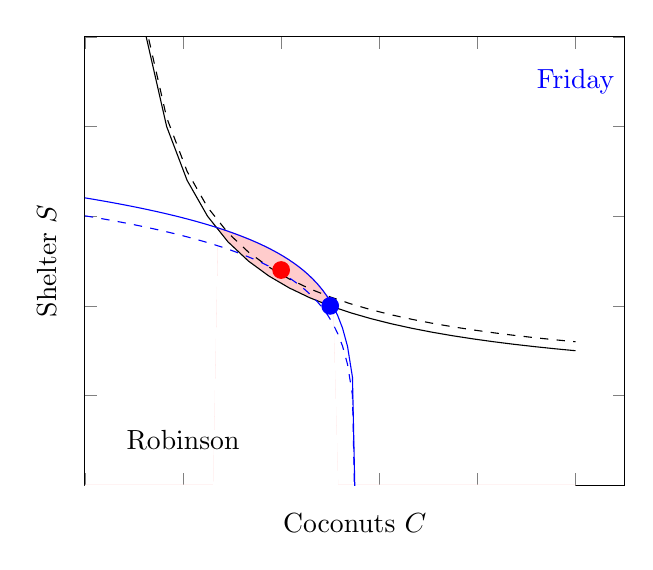
\begin{tikzpicture}
\begin{axis}[yticklabels={,,}, xticklabels={,,},xlabel={Coconuts $C$}, ylabel={Shelter $S$}, ymin=0,ymax=10,xmin=0]

\addplot[fill, red, opacity = 0.2, domain=0:1, samples=100]
{ln(-9*x+5)+4.8 > (1/x+2) ? ln(-9*x+5)+4.8 : 0} \closedcycle;

\addplot[fill, white, domain=0:1, samples=100]
{ln(-9*x+5)+4.8 > (1/x+2) ? (1/x+2) : 0} \closedcycle;

\addplot[mark=*, blue, mark size=3pt, domain=0:100]
coordinates {(0.5,4)};

\addplot[mark=*, red, mark size=3pt, domain=0:100]
coordinates {(0.4,4.8)};

\addplot[black, domain=0:1]
{1/x+2};

\addplot[blue, domain=0:1,samples=100]
{ln(-9*x+5)+4.8};

\addplot[black, domain=0:1, dashed]
{1/x+2.2};

\addplot[blue, domain=0:1,samples=100, dashed]
{ln(-9*x+5)+4.4};

% name markings
\addplot[black, domain=0:200]
coordinates {(0,0)} node at (axis cs:0.2,1) {\color{black} Robinson} node at (axis cs:1,9) {\color{blue} Friday};
\end{axis}
\end{tikzpicture}
\caption{Edgeworth Box of Robinson and \color{blue} Friday}
\end{figure}

At this red point, no further exchanges can make anyone better off without making any of them worse off.

Incidentally, it is also at this point that their MRSes are equal (recall the earlier condition we derived?)

\begin{figure}[ht!]
\begin{subfigure}[b]{0.5\textwidth}
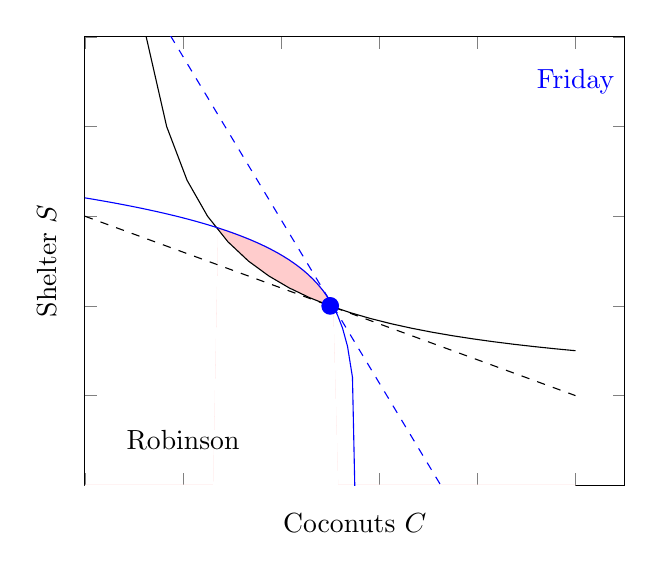
\begin{tikzpicture}
\begin{axis}[yticklabels={,,}, xticklabels={,,},xlabel={Coconuts $C$}, ylabel={Shelter $S$}, ymin=0,ymax=10,xmin=0]

\addplot[fill, red, opacity = 0.2, domain=0:1, samples=100]
{ln(-9*x+5)+4.8 > (1/x+2) ? ln(-9*x+5)+4.8 : 0} \closedcycle;

\addplot[fill, white, domain=0:1, samples=100]
{ln(-9*x+5)+4.8 > (1/x+2) ? (1/x+2) : 0} \closedcycle;

\addplot[mark=*, blue, mark size=3pt, domain=0:100]
coordinates {(0.5,4)};

\addplot[black, domain=0:1]
{1/x+2};

\addplot[blue, domain=0:1, dashed]
{-18.1983*x+13.2};

\addplot[black, domain=0:1, dashed]
{-4.0016*x+6};

\addplot[blue, domain=0:1,samples=100]
{ln(-9*x+5)+4.8};

% name markings
\addplot[black, domain=0:200]
coordinates {(0,0)} node at (axis cs:0.2,1) {\color{black} Robinson} node at (axis cs:1,9) {\color{blue} Friday};
\end{axis}
\end{tikzpicture}
\end{subfigure}
\hspace{2ex}
\begin{subfigure}[b]{0.5\textwidth}
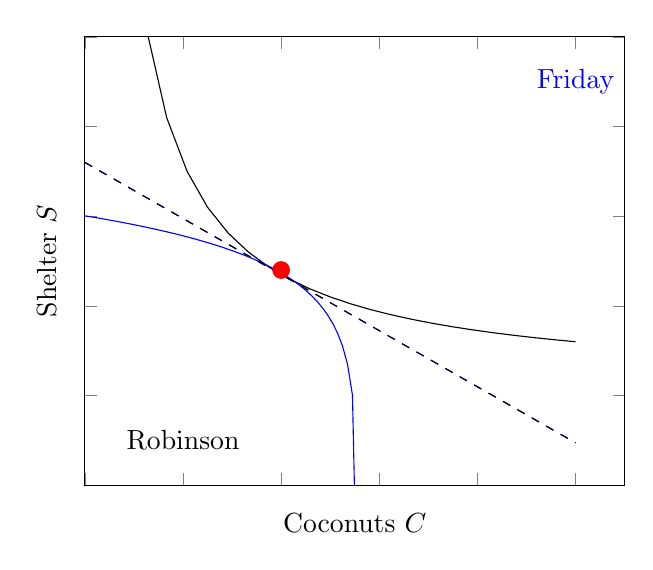
\begin{tikzpicture}
\begin{axis}[yticklabels={,,}, xticklabels={,,},xlabel={Coconuts $C$}, ylabel={Shelter $S$}, ymin=0,ymax=10,xmin=0]

\addplot[mark=*, red, mark size=3pt, domain=0:100]
coordinates {(0.4,4.8)};

\addplot[black, domain=0:1]
{1/x+2.2};

\addplot[blue, domain=0:1,samples=100]
{ln(-9*x+5)+4.4};

\addplot[blue, domain=0:1, dashed]
{-6.2539*x + 7.2};

\addplot[black, domain=0:1, dashed]
{-6.2539*x + 7.2};

% name markings
\addplot[black, domain=0:200]
coordinates {(0,0)} node at (axis cs:0.2,1) {\color{black} Robinson} node at (axis cs:1,9) {\color{blue} Friday};
\end{axis}
\end{tikzpicture}
\end{subfigure}
\caption{When indifference curve are tangent to each other, the MRSes are equal and we have exchange efficiency}
\end{figure}

\subsection{Production Efficiency}

Here, we answer the question, "How much should Robinson labor for coconuts?\footnote{A similar argument can be made for Robinson's labor for shelter, Friday's labor for coconuts and Friday's labor for shelter}"

Again, we measure cost and benefits. Here, we assume that Robinson is already at productive efficiency. Then, if he works $\epsilon$ more hours to gather coconuts,

\begin{table}[ht!]
\begin{longtable}{c|c}
\hline
 & Robinson \\
\hline
Marginal Benefit & $U'_{R,C} F'_{C,L} \epsilon$ \\
Marginal Cost & $U'_{R,Z} \epsilon$ \\
\hline
\end{longtable}
\caption{Marginal Costs and Benefits for Robinson}
\end{table}

His marginal benefit of working $\epsilon$ more hours is the marginal utility per coconut, times the number of coconuts manufactured. The number of coconuts manufactured is the marginal productivity of labor for coconuts times the number of hours worked. 

Recall the production functions $Y_C$ and $Y_S$, where $Y_C = F_C(L_C, N_C)$. Imagine this as a factory that produces coconuts. Robinson needs to work at the factory to produce coconuts. So if Robinson works $\epsilon$ hours at the factory, he will produce $F'_{C,L} \epsilon$ where $F'_{C,L}$ is the additional number of coconuts produced per hour of labor. 

If the number of hours Robinson works is already optimal, then marginal benefit of working should equal marginal cost.

\begin{align*}
\mathrm{MB} = \mathrm{MC}\\
U'_{R,C} F'_{C,L} \epsilon &= U'_{R,Z} \epsilon \\
\frac{U'_{R,C}}{U'_{R,Z}} &= F'_{C,L}
\end{align*}

This means that the number of coconuts Robinson is willing to give up for an extra hour of leisure must equal the number of coconuts one can produce using an extra hour of labor. 

What if 

\[ \frac{U'_{R,C}}{U'_{R,Z}} > F'_{C,L} \]

Then, Robinson losing the equivalent utility of giving up $\frac{U'_{R,C}}{U'_{R,Z}}$ coconuts, which is more than what he's earning for the last hour of work. That's not good right?

\subsection{Land Efficiency}

Now we answer the question, "How much land should Robinson use for producing coconuts vs. shelters?" Again, we look at marginal benefits and costs.

Suppose Robinson transfers $\epsilon$ land from shelter production to coconut production\footnote{Again, similar arguments can be made for Friday as well}

\begin{table}[ht!]
\begin{longtable}{c|c}
\hline
 & Robinson \\
\hline
Marginal Benefit & $U'_{R,C} F'_{C,N} \epsilon$ \\
Marginal Cost & $U'_{R,S} F'_{S,N} \epsilon$ \\
\hline
\end{longtable}
\caption{Marginal Costs and Benefits for Robinson}
\end{table}

The marginal benefit is the marginal utility per coconut times the number of additional coconuts. The number of additional coconuts is the marginal product of land for coconuts, times the amount of additional land dedicated to coconut production. A similar argument applies for marginal cost.

Again, equating marginal benefit and cost because in order to maximize utility, these two must be equal, we get

\[ \frac{U'_{R,C}}{U'_{R,S}} = \frac{F'_{C,N}}{F'_{S,N}} \]

This is the condition for land efficiency.

\section{Markets}

\subsection{Information Problem of Central Planning}

We realize that we have to solve many simultaneous equations to achieve efficiency in exchange, production, and land. 

\begin{itemize}

\item For exchange, we have to make sure that distribution between coconuts and shelter, shelter and leisure, and leisure and coconuts are optimal. That's 3 equations.
\item For production, we have to ensure that Robinson's distribution of labor between coconut and leisure, shelter and leisure, and Friday's distribution of labor between coconut and leisure, shelter and leisure are optimal. That's 4 equations.
\item For land efficiency we have to make sure that both people are distributing land efficiently. That's 2 equations.
\end{itemize}

For a very unrealistic model of two people on a lonely little island with the barest minimal resources and an absolutely monotonous diet, we already have to solve 9 simultaneous equations. What about real economies? There will simply be too much information for any person or government to process centrally.

Enter markets.

\subsection{Product Market for Exchange Efficiency}

Instead of the government (or in the case of many games, you the player) deciding how much each individual should consume, let the market do that job!

Robinson will trade shelter for coconuts until

\[ \frac{U'_{R,S}}{U'_{R,C}} = P_C \]

Similarly, Friday will trade shelter for coconuts until

\[ \frac{U'_{F,S}}{U'_{F,C}} = P_C \]

This results in

\[ \frac{U'_{R,S}}{U'_{R,C}} = \frac{U'_{F,S}}{U'_{F,C}} \]

$P_C$ is not set externally, but arises due to demand and supply. If $P_C$ was too high, there will be over-supply of coconuts, driving prices down and vice versa. 

All that's happening here is the creation of a market. If similar markets existed for all goods (eg. Shelter), then there will be exchange efficiency for all goods.

\subsection{Labor Market for Production Efficiency}

Now imagine that both Robinson and Friday goes to a coconut factory to production coconuts ($F_C$), and a shelter factory to produce shelters ($F_S$). Let's say both Robinson and Friday gets paid wages.

In that case, Robinson will work until

\[\frac{U'_{R,Z}}{U'_{R,C}} = w\]

The same applies for Friday.

There will be demand for labor until

\[ w = F'_{C,L}\] 

or the Marginal Product of Labor for coconuts.

This yields production efficiency:

\[\frac{U'_{R,Z}}{U'_{R,C}} = F'_{C,L}\] 

\subsection{Land Market for Land Efficiency}

Now suppose that there is land ownership, and land is rented out at rental $r$ shelters. 

Shelter producers will demand land until the Marginal Product of Land for shelters equals rent in terms of shelters.

\[ F'_{S,N} = r \]

Coconut producers will demand land until the Marginal Product of Land for coconuts equals rent in terms of shelters times price of coconuts in terms of shelters.

\[ P_C F'_{C,N} = r\]


Since $P_C = \frac{U'_{R,S}}{U'_{R,C}}$, 

\begin{align*}
\left( \frac{U'_{R,S}}{U'_{R,C}} \right) F'_{C,N} &= F'_{S,N} \\
\frac{U'_{R,S}}{U'_{R,C}} &= \frac{F'_{S,N}}{F'_{C,N}}
\end{align*}

Again, markets lead to efficiency.

\section{Implications on the Role of the Government}

This implies that the government has two main roles:

\begin{itemize}
\item Establish well defined property rights
\item Establish competitive markets for all goods and services
\end{itemize}

If you want to read more about this, I suggest Adam Smith and Hayek. Hayek in particular is very enlightening. 

\subsection{Market Failures}

Our analysis so far assumes that the market is without friction. However, it is your responsibility as a economist to realize that the market can fail sometimes, and to recognize that there is a legitimate role for intervention in these cases. 

Lots of people frequently criticize economists for believing that markets always work well. Truth to be told, no economist worthy of that title will dare to claim that. However, as much as I'd love to talk about market failures, we'll leave this topic to a later time. 


\end{document}